\documentclass[10pt,a4paper]{article}

\usepackage[utf8]{inputenc}
\usepackage[english,russian]{babel}
\usepackage{amsmath}
\usepackage{amsfonts}
\usepackage{amssymb}
\usepackage{textcomp}
\usepackage{graphicx}
\usepackage{hyperref}

\usepackage[margin=17mm]{geometry}

\begin{document}

\title{Скрытые Марковские модели переменного порядка для анализа данных
  ChIP-seq}
\author{Атаманова Анна, кафедра системного программирования СПбГУ, \url{anne.atamanova@gmail.com}}

\maketitle

\begin{abstract}
  Здесь нужно кратко описать суть работы и результаты.
\end{abstract}

\section{Введение}

Дезоксирибонуклеиновая кислота (ДНК) является своеобразным кодом жизни. Эта молекула хранит и передает генетическую программу развития и функционирования живого организма.
В то же время, все функции ДНК зависят от ее соединений с белками.
Поэтому, изучение ДНК-белковых взаимодействий актуально и привлекательно.
Chip-seq (chromatin immunoprecipitation - sequencing)\cite{Johnson2007} является одним из современных методов, позволяющим выделить участки ДНК связанные с конкретным белком (одинаково применим к разным белкам).
Однако, по понятным причинам (сложный биологический эксперимент), погрешность данного метода не может быть нулевой, и безрассудная вера ему лишена смысла. По этому, обычно, к результатам подобных методов накладывается вероятностная модель. Конечно, это добавляет ряд существенных ограничений. Однако, в качестве неоспоримого плюса можно привести тот факт, что хорошо подобранная модель позволяет понять природу данных и изучить их свойства.

Итого, нашей задачей является нахождение модели по последовательности чисел выдаваемых Chip-seq.

В настоящее время, в качестве семейства искомых моделей, активное приминение находит HMM (Hidden Markov Model)\cite{Rabiner1989} второго порядка с Пуассоновским испусканием.
Данное семейство допускает предположение о том, что каждое состояние (наличие/отсутствие белка в заданной части генома) завист только от одного предыдущего.
Можно ограничиться и более лояльным допущением о том, что состояние зависит от $n$ предыдущих состояний, однако такое допущение резко увеличивает сложность модели ($O(2\textsuperscript{n})$ параметров). Также, сложность заключается в подборе этого $n$ и переобучении в случае, если не все состояния имеют одинаковые длины контекстов зависимости.
Последннее замечание подводит к идее использования VOHMM (Variable Order Hidden Markov Model)\cite{Wang2006}


\section{Скрытые марковские модели переменного порядка}

Марковский процесс порядка $ m $ - это случайный процесс, эволюция которого в каждый момент времени зависит только от $ m-1 $ предыдущих состояний.

Другими словами, $ X = (x_{1}, x_{1}, ..., x_{T}) $ является марковской цепью порядка $ m $,
если $ p(x_{t}|x_{1}^{t-1}) = p(x_{t}|x_{t-m+1}^{t-1})$ 

Таким образом, каждое следующее состояние определяется контекстом длины $ m-1 $ и вероятностями перехода из него.

Скрытая марковская модель предполагает, что, помимо всего прочего, каждое состояние задает свою вероятностною модель (например, гауссиан), а в качестве наблюдений поступают не сами состояния, а лишь испускания из них $y_{1},...,y_{T}$ (\ref{ris:image}- пример HMM порядка 2). 
\begin{figure}[hbtp]
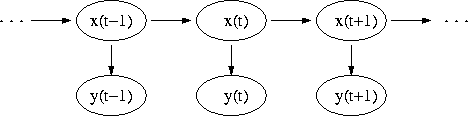
\includegraphics[scale=0.4]{Hmm_temporal_bayesian_net.png}
\centering
\caption{HMM order 2}
\label{ris:image}
\end{figure}


Скрытая марковская модель переменного порядка - обобщение HMM разрешающее иметь контекстам разные длины.
 
Итого, скрытая марковская модель переменного порядка определяется контекстами, вероятностными распределениями переходов и верояностными распределениями испусканий для каждого состояния.

Перейдем к обучению модели по цепочке наблюдений.

Обычно обучение $ n-hmm$ $ m $-го порядка сводится к $ n^{m}-hmm второго порядка$, котрая обучается алгоритмом Баума-Велха (частный случай EM алгоритма, который итеративно максимизирует правдоподобие модели).

Для хранения контекстов используется дерево (бор), в котором вершины являются строками, ребра буквами. Корень - это пустой контекст, а каждый ребенок вершины является уточнением контекста родителя на состояние ребра. 
Итого, каждая внутренняя вершина имеет ровно n потомков. Листья - главные контексты. 

Заметим, что, если дети какой-то вершины имеют одинаковые вероятности переходов, то они контекст вершины не уточняют, и их можно обрезать.

Так же заметим, что достаточно хранить только листья и распределение переходов на них, и, в случае необходимости, пересчитывать его на внутренние вершины 

$ p(q|s) = \frac{\sum_{c \in C(s)} {p(q|c)}}{\sum_q\sum_{c \in C(s)} {p(q|c)}} $ ,

где $ q $ - состояние, $ C(s )$ - все листья (контексты), являющися потомками $ s $

Изначально берется полное дерево некоторой фиксированной глубины $m$.

Обучение модели по цепочки наблюдений происходит с помощью чередования EM-алгоритма и обрезания дерева. 

EM-часть максимизирует правдоподобие модели алгоритмом Баума-Велха

Обрезание дерева производится нахождением родителей лиистьев, все потомки которых имеют близкие распределения переходов. Все дети такой вершины ликвидируются, а сама вершина становится новым контекстом. Критерием сравнения распределений переходов служит расстояние Кульбака-Лейблера. 

Инициализация каждого следующего EM ведется с помощью пересчета распределения переходов на новые контексты.

Изначальная инициализация производится путем построения цепочки состояний алгоритмом $ k $-means по наблюдениям (где $k=n$) и частотной оценкой вероятности переходов на ней.

\section{Оценка модели}

\section{Заключение}

\bibliographystyle{plain}
\bibliography{references}

\end{document}
